\documentclass[11pt]{article}
\usepackage[margin=1in]{geometry}
\usepackage{times}
\usepackage{multicol}
\usepackage{titlesec}
\usepackage{enumitem}
\usepackage{setspace}
\usepackage{titling}
\usepackage{authblk}
\usepackage{graphicx}
\usepackage{caption}
\usepackage{hyperref}
\usepackage{url}

% Section formatting
\titleformat{\section}{\large\bfseries}{\thesection}{1em}{}
\titleformat{\subsection}{\normalsize\bfseries}{\thesubsection}{1em}{}
\titleformat{\subsubsection}{\normalsize\itshape}{\thesubsubsection}{1em}{}

% Remove numbering from sections
\setcounter{secnumdepth}{0}

% Remove page numbers/headers per style guidance (added at typesetting)
\pagestyle{plain}

% Title and metadata (authors/affiliations left blank for double-blind review)
\title{Automated Cyber Range Infrastructures for Securing Tomorrow: Lessons from Range42}
\author{} % Fill after review per CyCon guidance
\date{}   % Leave empty for submission

\begin{document}
\maketitle

\begin{abstract}
The future of cyber conflict demands training and testing platforms that anticipate tomorrow’s threats rather than replicate yesterday’s incidents. This paper presents Range42, an open cyber range developed by the National Cybersecurity Competence Center (NC3) under the Luxembourg House of Cybersecurity together with DIGISQUAD. Designed as a flexible, automated platform, Range42 lowers barriers to building realistic and reproducible training environments while fostering collaborative research and development.

Our research introduces two core contributions. First, we describe an extensible inventory system of vulnerable and misconfigured environments. With over 100 curated CVEs and misconfigurations identified and approximately 20 already deployable, this system enables structured reproduction of real-world attack surfaces for controlled experiments. Second, we detail an orchestration framework capable of deploying multi-subnet infrastructures, making it possible to simulate complex enterprise-grade networks with isolation and fidelity.

We outline the automation pipeline—including Proxmox integration, Ansible-driven provisioning, container and VM deployment, and Tailscale-enabled zero-trust connectivity—and assess its ability to create scalable, reusable, and secure scenarios.

We conclude that open, automated cyber ranges such as Range42 are essential to “securing tomorrow.” They enable hands-on training, accelerate scenario design, and provide accessible platforms for testing defensive strategies against emerging threats.
\end{abstract}

\section{Introduction}
Cyber threats evolve faster than training and evaluation methodologies. To \emph{secure tomorrow}, cyber ranges must enable realistic, reproducible, and rapidly composed environments that reflect emerging attack surfaces and defensive strategies. We present \textbf{Range42}, an open cyber range platform emphasizing automation, flexibility, and collaboration. Our contributions are: (1) an extensible inventory of vulnerable/misconfigured systems for research-grade reproducibility; and (2) an orchestration framework for deploying multi-subnet infrastructures approximating enterprise topologies. We outline our automation pipeline and report lessons for scalability, isolation, and openness.

\section{Background and Related Work}
Prior work spans commercial, academic, and government cyber ranges; however, many platforms are closed or bespoke, limiting reproducibility, comparability, and community validation. Open, automated ranges reduce barriers for training, experimentation, and replication of results. We position Range42 in this landscape and identify gaps in open orchestration, inventory standardization, and zero-trust access for distributed exercises.

\section{System Architecture}
Range42 integrates: (i) Proxmox for VM lifecycle; (ii) Ansible for idempotent provisioning; (iii) containers and VMs for workload flexibility; and (iv) Tailscale (WireGuard-based) for identity-aware, zero-trust connectivity. Figure~\ref{fig:arch} sketches the build--deploy--run pipeline and control surfaces.
\begin{figure}[h]
\centering
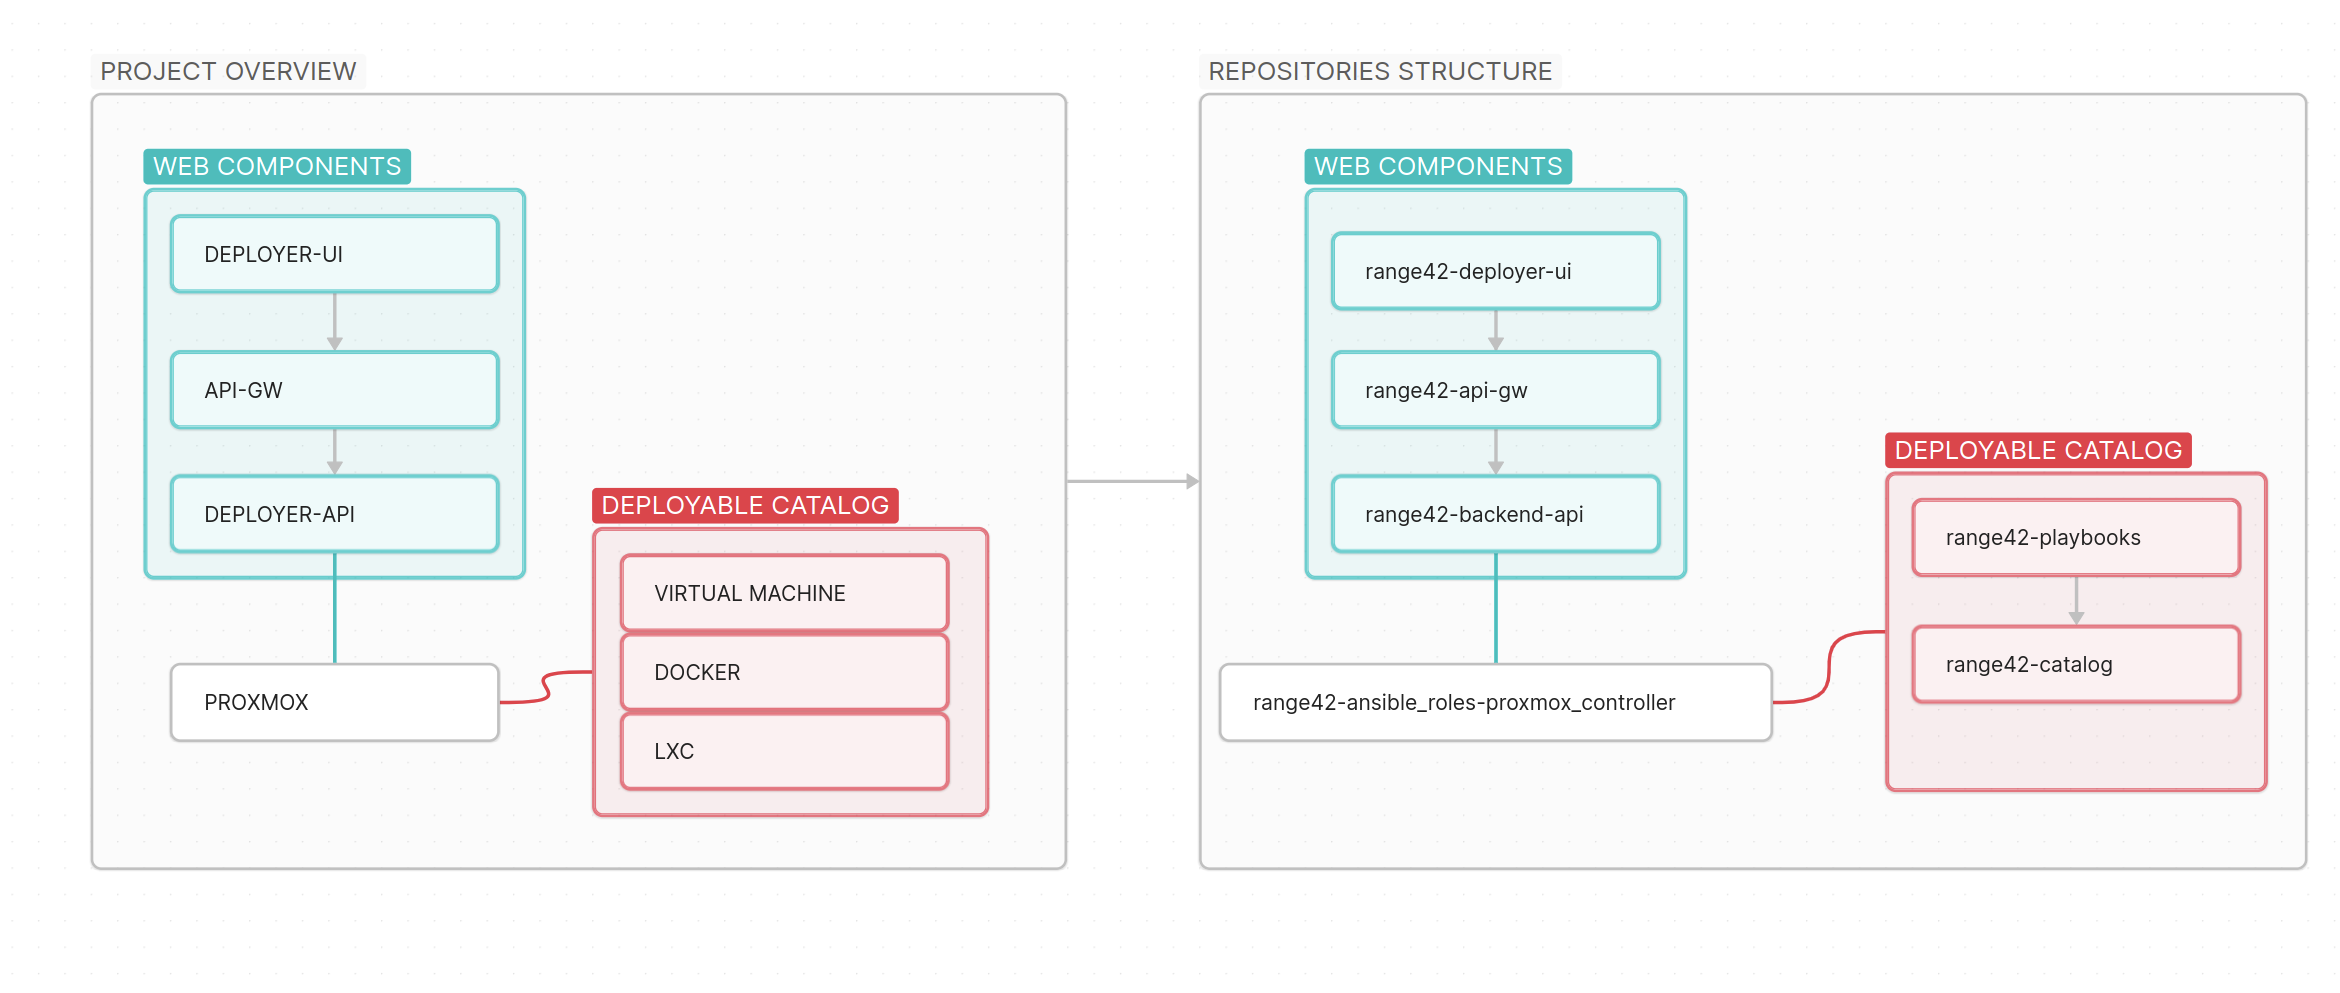
\includegraphics[width=0.9\linewidth]{images/diagrams/architecture.png}
\caption{High-level Range42 architecture and automation pipeline (placeholder).}
\label{fig:arch}
\end{figure}

\section{Vulnerability and Misconfiguration Inventory}
We curate an inventory of $\sim$100 CVEs/misconfigurations (with $\sim$20 currently deployable), using build descriptors and snapshotting to balance reproducibility with support for proprietary or atypical systems. The design supports traceability, variant creation, and controlled risk exposure during exercises.

\section{Multi-Subnet Orchestration}
Realistic exercises require routed, segmented networks. Our orchestration composes multi-subnet topologies with per-segment policy, enabling blue/red/purple-team exercises and layered defenses. We discuss challenges (addressing, routing, firewall policy, performance) and our mitigation strategies using Proxmox APIs and Ansible roles.

\section{Evaluation}
We evaluate deployment time, reproducibility, and scale (concurrent labs/users) across representative scenarios. Where quantitative metrics are constrained by resource ceilings, we complement with qualitative feedback from instructors and operators. We report failure modes and remedies observed during pilot training events.

\section{Discussion}
We reflect on security trade-offs (fidelity vs.\ containment), operational debt (image sprawl, secret handling), and governance (open contributions, quality gates). We argue that openness is a force multiplier for resilience: it improves scrutiny, reuse, and portability across institutions.

\section{Future Work}
Planned work includes: expanding inventory coverage; advancing a visual lab designer; integrating malware analysis/forensics workflows; and supporting richer hybrid topologies. We also plan a unified scenario descriptor (YAML/JSON) to drive the gateway/orchestrator for end-to-end reproducibility.

\section{Conclusion}
Open, automated ranges like Range42 help \emph{secure tomorrow} by enabling hands-on research and training at scale. Our contributions---a reproducible inventory and multi-subnet orchestration---demonstrate a practical path to scalable, high-fidelity, and community-driven cyber range operations.

\bibliographystyle{IEEEtran}
\begin{thebibliography}{99}
\bibitem{proxmox} Proxmox VE. Available: \url{https://www.proxmox.com/}
\bibitem{ansible} Ansible Documentation. Available: \url{https://docs.ansible.com/}
\bibitem{docker} Docker Documentation. Available: \url{https://docs.docker.com/}
\bibitem{tailscale} Tailscale Documentation. Available: \url{https://tailscale.com/kb/}
\bibitem{ieee} IEEE Editorial Style Manual. Available: \url{https://journals.ieeeauthorcenter.ieee.org/}
\end{thebibliography}

\end{document}
